%\section{Physical Human Factors Report: Tristan Griffith}
\rhead{\today}
\begin{center}
{\large  Tristan Griffith}\\
\vspace{2mm}
{\large Dr. James Hubbard Jr.}
\noindent\rule{\textwidth}{2pt}
\end{center}
\setcounter{section}{1}

%\begin{wrapfigure}{r}{0.45\textwidth}
%\centering
%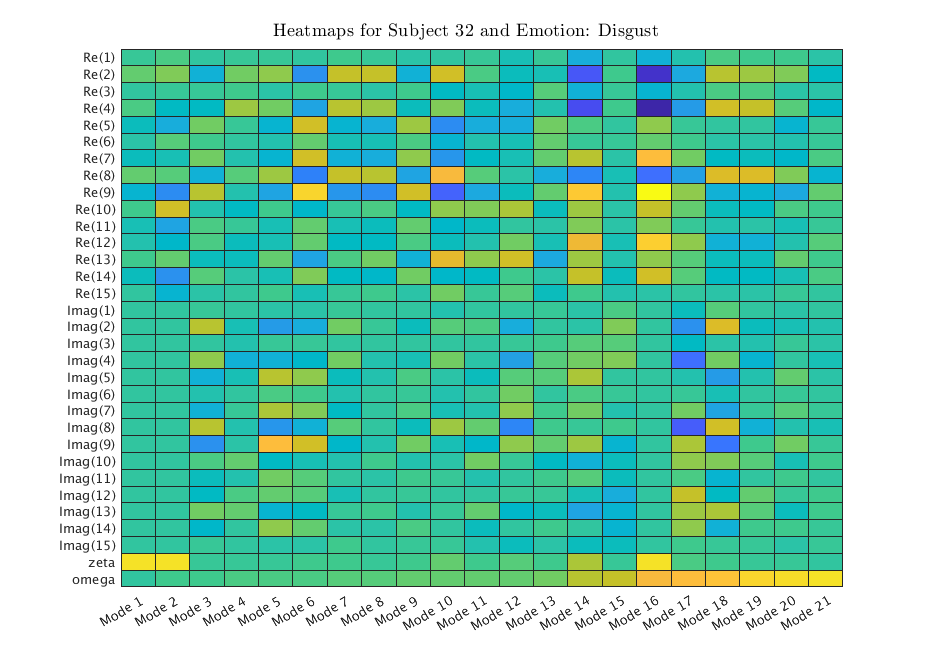
\includegraphics[scale=.3]{../../../figures/demo_map.png} 
%\caption{Modal Heatmap for Subject 32}
%\end{wrapfigure}
\subsection{Introduction}
We inquire concerning the nature of traveling waves in the brain. Under this head there are three points of inquiry:
\begin{enumerate}
\item Whether the brain has traveling waves?
\item Whether fMRI waves are connected to EEG waves?
\item If traveling waves exist, are they relevant to clinical outcomes?
\end{enumerate}
\subsection{Whether the brain has traveling waves?}
\textbf{Objection 1:} Prior work has shown repeated decoherence among spatially distributed recordings of brain activity. Theta oscillations in humans are postulated to have only local mechanisms \cite{doi:10.1152/jn.00409.2005}. 
\begin{displayquote}
 We found that, whereas nearby gated sites $(<20 \textit{mm})$ were often but not always coherent, distant gated sites were almost never coherent. Our results imply that there are local mechanisms for the generation of cortical theta.
\end{displayquote}
\textbf{Objection 2:} While inter-electrode spatial correlations in the gamma band have been discovered in animals, the same was not found in humans \cite{MENON199689}.
\begin{displayquote}
The findings suggest that the surface diameters of domains of spatially correlated activity underlying perceptual categorization in human gamma band ECoG are limited to less than 2 cm and that the intermittent synchronization observed across separations of 1 cm and 1.4 cm is not solely due to volume conduction. Thus, if such gamma band spatial patterns exist in the human brain, no existing technology would be capable of measuring them at the scalp, and subdural electrode arrays for cortical surface recording would have to have spacings under 5 mm.
\end{displayquote}
\textbf{Objection 3:} Using statistical methods, EEG coherence was found to decline substantially in space across all frequency bands \cite{BULLOCK1995161}.
\begin{displayquote}
In both the subdural surface samples and those from temporal lobe depth electrode arrays coherent declines with distance between electrodes of the pair, on the average quite severely in millimeters. This is nearly the same for all frequency bands. 
\end{displayquote}
\textbf{On the contrary,} it has been found most recently that when \textbf{phase} is considered as part of the spatial coherence, traveling and standing waves are observed across a broad spectrum for most subjects \cite{ZHANG20181269}.





%\begin{displayquote}
%The class of monotone DNF expressions is learnable via an algorithm $B$ that uses $L=L(h,d)$ calls of examples and $dt$ calls of oracle, where $d$ is the degree of the DNF expression $f$ to be learnt and $t$ the number of variables.
%\end{displayquote}


%\begin{wrapfigure}{r}{0.55\textwidth}
%\centering
%\includegraphics[scale=.5]{../figures/complexity.png} 
%\caption{The Error-Complexity Trade Off}
%\end{wrapfigure}

